\documentclass[aspectratio=169]{beamer}

\usetheme{Boadilla}
\usefonttheme{professionalfonts}
\setbeamertemplate{navigation symbols}{}
\setbeamertemplate{itemize items}[circle]
\setbeamertemplate{enumerate items}[default]
\setbeamertemplate{headline}{}

\usepackage[utf8]{inputenc}
\usepackage[T1]{fontenc}
\usepackage{lmodern}
\usepackage{amsmath}
\usepackage{booktabs}
\usepackage{tabularx}
\usepackage{array}
\usepackage{hyperref}
\usepackage[strings]{underscore}
\usepackage{listings}
\usepackage{tikz}
\usetikzlibrary{arrows.meta,positioning,fit,calc,shapes.geometric}
\usepackage{xcolor}

\definecolor{courseblue}{HTML}{12355B}
\definecolor{coursegold}{HTML}{C98A2E}
\definecolor{courseice}{HTML}{EEF3F8}
\definecolor{coursegreen}{HTML}{2F6B4F}
\definecolor{coursegray}{HTML}{4B5563}
\definecolor{codebg}{HTML}{F7F9FC}
\definecolor{codecomment}{HTML}{5E6C84}
\definecolor{codestring}{HTML}{0B6E4F}

\setbeamercolor{palette primary}{bg=courseblue,fg=white}
\setbeamercolor{palette secondary}{bg=coursegold,fg=white}
\setbeamercolor{palette tertiary}{bg=courseblue,fg=white}
\setbeamercolor{palette quaternary}{bg=coursegold,fg=white}
\setbeamercolor{structure}{fg=courseblue}
\setbeamercolor{frametitle}{bg=courseice,fg=courseblue}
\setbeamercolor{title}{fg=courseblue}
\setbeamercolor{block title}{bg=courseblue,fg=white}
\setbeamercolor{block body}{bg=courseice,fg=black}
\setbeamercolor{normal text}{fg=black,bg=white}
\setbeamercolor{alerted text}{fg=coursegold}

\setbeamerfont{footline}{size=\scriptsize}

\setbeamertemplate{footline}{
  \leavevmode
  \hbox{
    \begin{beamercolorbox}[wd=.33\paperwidth,ht=2.8ex,dp=1.2ex,leftskip=0.8em]{palette primary}%
      University of Trieste
    \end{beamercolorbox}%
    \begin{beamercolorbox}[wd=.49\paperwidth,ht=2.8ex,dp=1.2ex,center]{palette tertiary}%
      \coursename{} \textbar{} \coursecode
    \end{beamercolorbox}%
    \begin{beamercolorbox}[wd=.18\paperwidth,ht=2.8ex,dp=1.2ex,right,rightskip=0.8em]{palette secondary}%
      \insertframenumber{} / \inserttotalframenumber
    \end{beamercolorbox}%
  }
}

\hypersetup{
  colorlinks=true,
  linkcolor=courseblue,
  urlcolor=coursegreen
}

\lstdefinestyle{coursepython}{
  language=Python,
  basicstyle=\ttfamily\footnotesize,
  keywordstyle=\color{courseblue}\bfseries,
  commentstyle=\color{codecomment}\itshape,
  stringstyle=\color{codestring},
  showstringspaces=false,
  columns=fullflexible,
  keepspaces=true,
  frame=single,
  framerule=0.6pt,
  rulecolor=\color{courseblue},
  backgroundcolor=\color{codebg},
  xleftmargin=0.4em,
  xrightmargin=0.4em,
  aboveskip=0.4em,
  belowskip=0.2em
}

\newcommand{\coursename}{Data-driven Systems Engineering}
\newcommand{\coursecode}{440MI / 305SM}
\newcommand{\coursefooter}{}

\newcommand{\learninggoals}[1]{
  \begin{block}{Learning goals}
  #1
  \end{block}
}

\newcommand{\repoactivity}[1]{
  \begin{block}{Repo activity}
  #1
  \end{block}
}

\newcommand{\readinglist}[1]{
  \begin{block}{Papers and materials}
  {\footnotesize #1}
  \end{block}
}

\newcommand{\coursecontextframe}[5]{
  \begin{frame}{Course Map and Running Cases}
  \centering
  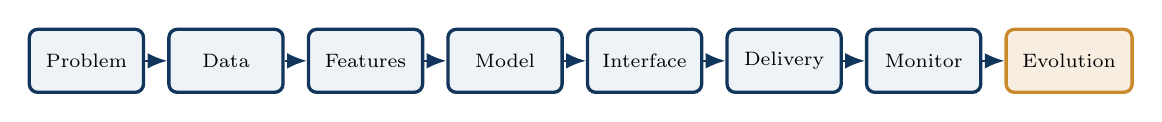
\begin{tikzpicture}[node distance=0.28cm]
  \node[flowbox, minimum width=1.45cm, minimum height=0.8cm] (problem) {\scriptsize Problem};
  \node[flowbox, minimum width=1.45cm, minimum height=0.8cm, right=of problem] (data) {\scriptsize Data};
  \node[flowbox, minimum width=1.45cm, minimum height=0.8cm, right=of data] (features) {\scriptsize Features};
  \node[flowbox, minimum width=1.45cm, minimum height=0.8cm, right=of features] (model) {\scriptsize Model};
  \node[flowbox, minimum width=1.45cm, minimum height=0.8cm, right=of model] (interface) {\scriptsize Interface};
  \node[flowbox, minimum width=1.45cm, minimum height=0.8cm, right=of interface] (delivery) {\scriptsize Delivery};
  \node[flowbox, minimum width=1.45cm, minimum height=0.8cm, right=of delivery] (monitor) {\scriptsize Monitor};
  \node[accentbox, minimum width=1.6cm, minimum height=0.8cm, right=of monitor] (evolution) {\scriptsize Evolution};
  \foreach \a/\b in {problem/data,data/features,features/model,model/interface,interface/delivery,delivery/monitor,monitor/evolution} {
    \draw[arrow] (\a) -- (\b);
  }
  \end{tikzpicture}

  \vspace{0.5em}
  \begin{block}{Today in the course}
  \textbf{Focus:} #1

  \textbf{Bridge:} #2
  \end{block}

  \begin{columns}[T]
  \column{0.48\textwidth}
  \begin{block}{Fraud case}
  {\footnotesize #3}
  \end{block}
  \column{0.48\textwidth}
  \begin{block}{Pasteurization case}
  {\footnotesize #4}
  \end{block}
  \end{columns}

  \vspace{0.3em}
  {\footnotesize \textbf{Course thread:} #5}
  \coursefooter
  \end{frame}
}

\newcommand{\classclosingframe}[4]{
  \begin{frame}{From This Class to the Next}
  \begin{block}{What stays with us}
  #1
  \end{block}

  \begin{columns}[T]
  \column{0.48\textwidth}
  \begin{block}{Project use}
  {\footnotesize #2}
  \end{block}
  \column{0.48\textwidth}
  \begin{block}{Next connection}
  {\footnotesize #3}
  \end{block}
  \end{columns}

  \vspace{0.3em}
  {\footnotesize \textbf{Course thread:} #4}
  \coursefooter
  \end{frame}
}

\tikzset{
  flowbox/.style={
    rounded corners=3pt,
    draw=courseblue,
    fill=courseice,
    very thick,
    minimum width=2.2cm,
    minimum height=0.9cm,
    align=center,
    font=\small
  },
  accentbox/.style={
    rounded corners=3pt,
    draw=coursegold,
    fill=coursegold!15,
    very thick,
    minimum width=2.2cm,
    minimum height=0.9cm,
    align=center,
    font=\small
  },
  arrow/.style={
    -{Latex[length=2.5mm,width=2mm]},
    thick,
    draw=courseblue
  }
}

\usepackage{amssymb}
\usetikzlibrary{decorations.pathreplacing}

\title{Class 14: Structured Data, Encoding, and Embeddings}
\author{\coursename}
\date{}

\begin{document}

\frame{\titlepage \coursefooter}

\begin{frame}{Agenda}
\begin{itemize}
\item From data type to data structure: structured, semi-structured, unstructured.
\item Where each structure shows up in this repository's real services.
\item Why raw values must be encoded before a model can use them.
\item One-hot, ordinal, target, and cyclic encoding.
\item Encoding versus embedding as two different compression strategies.
\item Dimensionality reduction (PCA) as feature extraction after encoding.
\end{itemize}
\coursefooter
\end{frame}

\begin{frame}{From data type to data structure}
\begin{itemize}
\item Class 13 asked whether data is tabular, time series, spectral, or image.
\item This class asks a orthogonal question: how organized is it, structured, semi-structured, or unstructured?
\item Any of the four data types from Class 13 can appear in any of these three organizational forms.
\item The organizational form determines how much encoding work is needed before a model can use the data at all.
\end{itemize}
\coursefooter
\end{frame}

\begin{frame}{Structured, semi-structured, and unstructured data}
\begin{tabularx}{\textwidth}{>{\bfseries}l X}
Structured & Fixed schema, fits directly into rows and columns: a CSV file or a SQL table. \\
Semi-structured & Has organization (keys, tags, nesting) but no fixed column schema: JSON logs, XML documents, API payloads. \\
Unstructured & No inherent schema at all: raw text, images, and audio waveforms. \\
\end{tabularx}
\coursefooter
\end{frame}

\begin{frame}{The taxonomy as a tree}
\centering
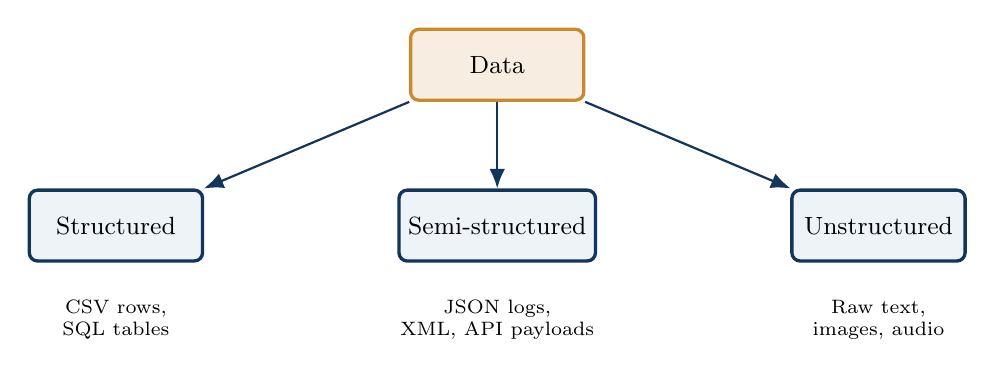
\begin{tikzpicture}[node distance=0.9cm and 0.6cm]
\node[accentbox] (root) {Data};
\node[flowbox, below left=1.1cm and 2.6cm of root] (s) {Structured};
\node[flowbox, below=1.1cm of root] (ss) {Semi-structured};
\node[flowbox, below right=1.1cm and 2.6cm of root] (u) {Unstructured};
\draw[arrow] (root) -- (s);
\draw[arrow] (root) -- (ss);
\draw[arrow] (root) -- (u);
\node[below=0.35cm of s, font=\scriptsize, align=center] {CSV rows,\\SQL tables};
\node[below=0.35cm of ss, font=\scriptsize, align=center] {JSON logs,\\XML, API payloads};
\node[below=0.35cm of u, font=\scriptsize, align=center] {Raw text,\\images, audio};
\end{tikzpicture}
\coursefooter
\end{frame}

\begin{frame}[fragile]{Semi-structured example: a streaming JSON event}
\begin{columns}[T]
\column{0.4\textwidth}
\begin{lstlisting}[basicstyle=\ttfamily\scriptsize, columns=fullflexible, keepspaces=true, frame=single, backgroundcolor=\color{codebg}, rulecolor=\color{courseblue!40}]
data: {
  "timestamp": 162.0,
  "batch_id": 1,
  "state": "Hold",
  "T": 71.987,
  "pH": 6.663,
  "Kappa": 4.79,
  "Mu": 1.624,
  "Tau": 0.978,
  "Q_in": 0.0,
  "Q_out": 0.0,
  "P": 1.199,
  "dTdt": -0.008
}
\end{lstlisting}
{\tiny One event emitted by the \texttt{/stream} endpoint of \texttt{pasteurization/serving.py} (batch 1, Hold phase); values rounded to three decimals.\par}
\column{0.56\textwidth}
\begin{itemize}\small
\item Each event is a self-describing object: every value is paired with the key that names it, so the record carries its own schema.
\item The schema is implicit, defined by the producer rather than enforced by the format. The same service returns a differently shaped object, \texttt{\{"error": "..."\}}, from \texttt{/point} when a request falls outside the batch range.
\item Converting the stream into structured data requires fixing a key set: each event becomes one sample $\mathbf{x}_t$ of the design matrix, with \texttt{timestamp} as the index and \texttt{state} as a categorical variable.
\end{itemize}
\end{columns}
\coursefooter
\end{frame}

\begin{frame}{Unstructured data}
\centering
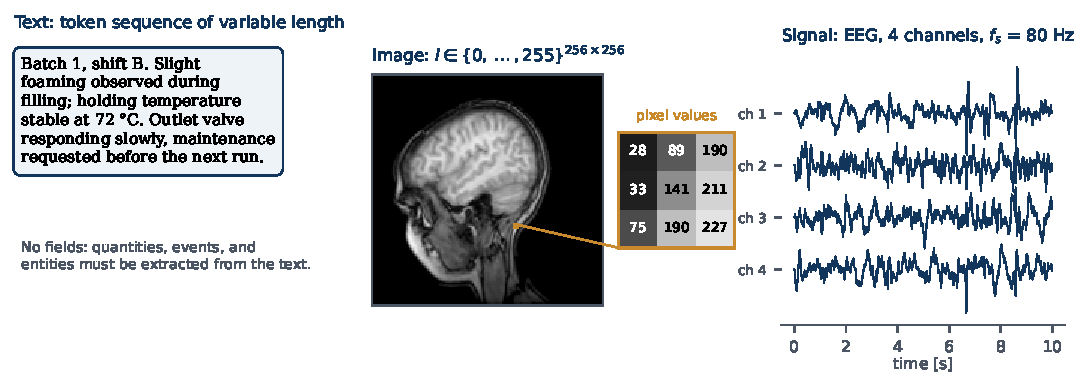
\includegraphics[width=\textwidth,height=0.52\textheight,keepaspectratio]{images/class14_unstructured_examples.pdf}

{\tiny Text: illustrative operator note. Image and signal: magnetic resonance imaging (MRI) slice and electroencephalography (EEG) recording from the Matplotlib sample data.\par}
\vspace{0.1em}
\begin{itemize}\footnotesize
\item No schema: meaning is not attached to named fields and must be extracted (quantities and entities in text, structures in images, events in signals).
\item The dimension is large and often variable (document length, image resolution, recording duration), so a learned representation, an embedding, is usually required.
\item Neither running case is unstructured, but production fraud and process-monitoring systems often complement their tabular core with free-text notes, images, or logs.
\end{itemize}
\coursefooter
\end{frame}

\begin{frame}{Representations: encoding and embedding}
\begingroup\small
A representation is a map $\phi: \mathcal{V} \to \mathbb{R}^{k}$ that assigns a numerical vector to each raw value $v \in \mathcal{V}$; every model operates on $\phi(v)$, never on $v$ itself. Two families of maps are distinguished:
\par\endgroup
\vspace{0.5em}
\begingroup\footnotesize
\begin{tabularx}{\textwidth}{>{\bfseries}l >{\raggedright\arraybackslash}X >{\raggedright\arraybackslash}X}
& \bfseries Encoding & \bfseries Embedding \\
\toprule
Construction & Designed a priori by the analyst & Learned from data (parameters estimated) \\
\addlinespace[0.3em]
Dimension & Determined by the variable, e.g.\ $k = K = |\mathcal{V}|$ & Chosen by the analyst, typically $k \ll K$ \\
\addlinespace[0.3em]
Structure & Often sparse & Dense \\
\addlinespace[0.3em]
Geometry & No similarity unless designed (one-hot: all values equidistant) & Similar values are mapped to nearby vectors \\
\addlinespace[0.3em]
Interpretability & Interpretable by construction & Generally not directly interpretable \\
\addlinespace[0.3em]
Typical use & Low-cardinality nominal, ordinal, and cyclic variables & High-cardinality categories, text, images \\
\bottomrule
\end{tabularx}
\par\endgroup
\coursefooter
\end{frame}

\begin{frame}{Encodings}
\begingroup\small
An encoding is a fixed map $\phi_{\mathrm{enc}}: \mathcal{V} \to \mathbb{R}^{k}$ specified before training. Its choice is determined by the cardinality $K = |\mathcal{V}|$ and the measurement scale of the variable.
\par\endgroup
\vspace{0.5em}
\begingroup\footnotesize
\renewcommand{\arraystretch}{1.5}
\begin{tabularx}{\textwidth}{>{\bfseries}l l c >{\raggedright\arraybackslash}X}
Encoding & $\phi_{\mathrm{enc}}(v)$ & $k$ & Appropriate when \\
\toprule
One-hot & $\mathbf{e}_v \in \{0,1\}^{K}$ & $K$ & Nominal scale, small $K$ \\
Ordinal & $r(v) \in \{1, \dots, K\}$, $r$ order-preserving & $1$ & Ordinal scale: the order is meaningful \\
Target & $\hat{\mu}_v = \dfrac{n_v \bar{y}_v + m\,\bar{y}}{n_v + m}$ & $1$ & Nominal scale, large $K$; estimated out-of-fold to avoid target leakage \\
Cyclic & $\big(\sin(2\pi v/P),\ \cos(2\pi v/P)\big)$ & $2$ & Periodic variables with period $P$ (e.g.\ hour of day, $P = 24$) \\
\bottomrule
\end{tabularx}
\par\endgroup
\vspace{0.4em}
{\scriptsize $n_v$: number of training samples with value $v$; $\bar{y}_v$: their mean target; $\bar{y}$: global mean; $m \ge 0$: smoothing weight, which shrinks $\hat{\mu}_v$ towards $\bar{y}$, more strongly when $n_v$ is small.\par}
\coursefooter
\end{frame}

\begin{frame}{Why encoding exists}
\begin{itemize}
\item Models compute with numbers; most raw variables (categories, labels, identifiers) are not numbers.
\item Encoding is the deliberate, documented choice of how a symbolic value becomes a numeric one.
\item A bad encoding can inject a false sense of order, leak information, or blow up dimensionality.
\item The right choice depends on cardinality (how many distinct values) and semantics (does order mean anything).
\end{itemize}
\coursefooter
\end{frame}

\begin{frame}{Encoding examples}
\centering
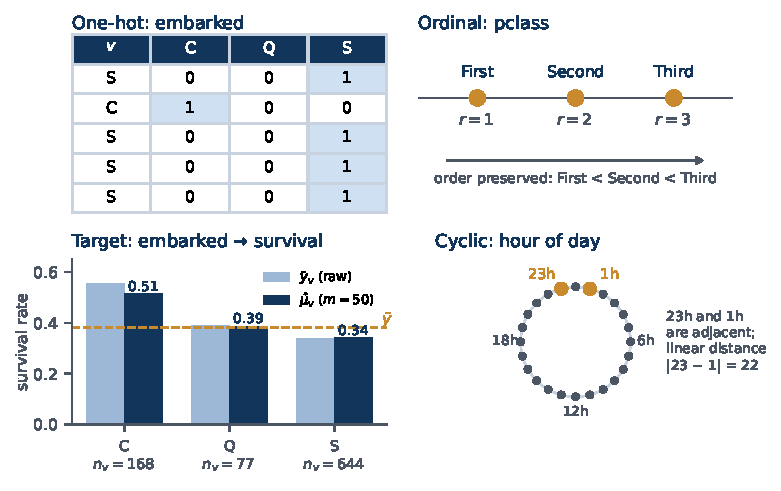
\includegraphics[width=\textwidth,height=0.72\textheight,keepaspectratio]{images/class14_encoding_examples.pdf}

\vspace{0.2em}
{\scriptsize Titanic data used in \texttt{notebooks/Class4\_DataEngineering.ipynb} (one-hot: first five samples; target: all samples with known port).\par}
\coursefooter
\end{frame}

\begin{frame}{Target encoding: a worked example}
\begingroup\small
\begin{columns}[T]
\column{0.47\textwidth}
\textbf{\color{courseblue} 1. Category means.} Each value $v$ is replaced by the mean target of the training samples with that value (Titanic, $y$ = survived).
\vspace{0.4em}

\begingroup\footnotesize\centering
\begin{tabular}{c r r c}
Port $v$ & $n_v$ & $\sum y$ & $\bar{y}_v$ \\
\toprule
C & 168 & 93 & 0.554 \\
Q & 77 & 30 & 0.390 \\
S & 644 & 217 & 0.337 \\
\midrule
All & 889 & 340 & $\bar{y} = 0.382$ \\
\bottomrule
\end{tabular}
\par\endgroup
\vspace{0.4em}
{The nominal column becomes a single numerical column, whatever the cardinality $K$; one-hot encoding would require $K$ columns.}

\column{0.5\textwidth}
\textbf{\color{courseblue} 2. Smoothing.} Rare values yield unreliable means; $\hat{\mu}_v$ is a weighted average of $\bar{y}_v$ and $\bar{y}$:
\[
\hat{\mu}_v = \frac{n_v \bar{y}_v + m\,\bar{y}}{n_v + m}, \qquad m = 50.
\]
\vspace{-0.6em}
\begingroup\footnotesize
\begin{itemize}
\item Port C ($n_v = 168$): $\hat{\mu}_C = \frac{93 + 50 \cdot 0.382}{218} = 0.514$.
\item Hypothetical port ($n_v = 2$, both survived): $\bar{y}_v = 1.0$, but $\hat{\mu}_v = \frac{2 + 19.1}{52} = 0.41$.
\end{itemize}
\par\endgroup
\vspace{0.3em}
\textbf{\color{courseblue} 3. Leakage control.} If a sample's own $y_i$ enters its encoding, the feature reveals the target. Training samples are therefore encoded out-of-fold; test samples use the means estimated on the training set.
\end{columns}
\par\endgroup
\coursefooter
\end{frame}

\begin{frame}{Embeddings}
\begingroup\small
An embedding is a learned map $\mathbf{z} = E^{\top}\phi_{\mathrm{enc}}(v)$, with $E \in \mathbb{R}^{K \times k}$ and $k \ll K$: each row of $E$ is the dense vector assigned to one value, estimated from data jointly with a model or through a dedicated objective (e.g.\ word2vec for text).
\par\endgroup
\vspace{0.3em}
\centering
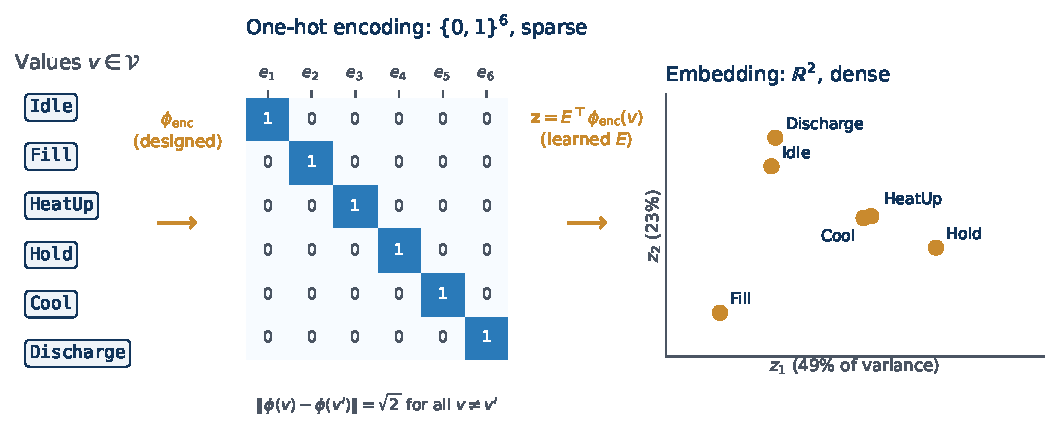
\includegraphics[width=\textwidth,height=0.56\textheight,keepaspectratio]{images/class14_encoding_vs_embedding.pdf}

\vspace{0.2em}
\begingroup\scriptsize\raggedright
One-hot encoding treats all categories as equidistant; the embedding places phases with similar sensor behaviour close together (HeatUp and Cool; Idle and Discharge). Embedding obtained by principal component analysis (PCA) of the standardized phase-wise means of nine sensor variables over 100 batches simulated with \texttt{synth\_sensors.py}.
\par\endgroup
\coursefooter
\end{frame}

\begin{frame}{word2vec: embeddings learned from context}
\begingroup\small
word2vec (Mikolov et al., 2013) learns the matrix $E$ from raw text under the \emph{distributional hypothesis}: words that occur in similar contexts have similar meanings.
\par\endgroup
\vspace{0.3em}
\centering
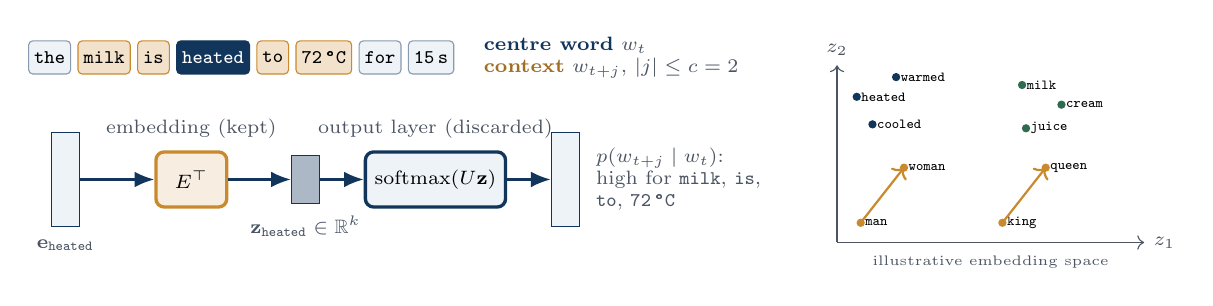
\begin{tikzpicture}[
  tok/.style={draw=courseblue!50, fill=courseice, rounded corners=1.5pt, inner sep=2pt, font=\scriptsize\ttfamily, minimum height=0.42cm},
  ctx/.style={tok, fill=coursegold!25, draw=coursegold},
  ctr/.style={tok, fill=courseblue, text=white, draw=courseblue},
  vec/.style={draw=courseblue, fill=courseice, minimum width=0.36cm, inner sep=0pt},
  lab/.style={font=\scriptsize, text=coursegray, align=center}
]
\node[tok] (w1) at (0,0) {the};
\node[ctx, right=0.08cm of w1] (w2) {milk};
\node[ctx, right=0.08cm of w2] (w3) {is};
\node[ctr, right=0.08cm of w3] (w4) {heated};
\node[ctx, right=0.08cm of w4] (w5) {to};
\node[ctx, right=0.08cm of w5] (w6) {72\,°C};
\node[tok, right=0.08cm of w6] (w7) {for};
\node[tok, right=0.08cm of w7] (w8) {15\,s};
\node[lab, right=0.25cm of w8, align=left] {\textcolor{courseblue}{\textbf{centre word}} $w_t$\\\textcolor{coursegold!80!black}{\textbf{context}} $w_{t+j}$, $|j| \le c = 2$};
\node[vec, minimum height=1.2cm] (oh) at (0.2,-1.55) {};
\node[lab, below=0.03cm of oh] {$\mathbf{e}_{\texttt{heated}}$};
\node[accentbox, minimum width=0.9cm, minimum height=0.7cm, font=\scriptsize] (E) at (1.8,-1.55) {$E^{\top}$};
\node[vec, minimum height=0.6cm, fill=courseblue!35] (z) at (3.25,-1.55) {};
\node[lab, below=0.03cm of z] {$\mathbf{z}_{\texttt{heated}} \in \mathbb{R}^{k}$};
\node[flowbox, minimum width=1.2cm, minimum height=0.7cm, font=\scriptsize] (sm) at (4.9,-1.55) {softmax$(U\mathbf{z})$};
\node[vec, minimum height=1.2cm] (out) at (6.55,-1.55) {};
\node[lab, right=0.08cm of out, align=left] {$p(w_{t+j} \mid w_t)$:\\high for \texttt{milk}, \texttt{is},\\\texttt{to}, \texttt{72\,°C}};
\draw[arrow] (oh) -- (E); \draw[arrow] (E) -- (z); \draw[arrow] (z) -- (sm); \draw[arrow] (sm) -- (out);
\node[lab, above=0.03cm of E] {embedding (kept)};
\node[lab, above=0.03cm of sm] {output layer (discarded)};
\begin{scope}[shift={(10.0,-2.35)}]
\draw[->, coursegray] (0,0) -- (3.9,0) node[right, lab] {$z_1$};
\draw[->, coursegray] (0,0) -- (0,2.25) node[above, lab] {$z_2$};
\foreach \x/\y/\w in {0.25/1.85/heated, 0.75/2.1/warmed, 0.45/1.5/cooled} {\fill[courseblue] (\x,\y) circle (1.5pt); \node[right, font=\tiny\ttfamily, inner sep=1.5pt] at (\x,\y) {\w};}
\foreach \x/\y/\w in {2.35/2.0/milk, 2.85/1.75/cream, 2.4/1.45/juice} {\fill[coursegreen] (\x,\y) circle (1.5pt); \node[right, font=\tiny\ttfamily, inner sep=1.5pt] at (\x,\y) {\w};}
\coordinate (m) at (0.3,0.25); \coordinate (wo) at (0.85,0.95);
\coordinate (k) at (2.1,0.25); \coordinate (q) at (2.65,0.95);
\foreach \p/\w in {m/man, wo/woman, k/king, q/queen} {\fill[coursegold] (\p) circle (1.5pt); \node[right, font=\tiny\ttfamily, inner sep=1.5pt] at (\p) {\w};}
\draw[->, coursegold, thick] (m) -- (wo); \draw[->, coursegold, thick] (k) -- (q);
\node[lab, font=\tiny, anchor=north] at (1.95,-0.05) {illustrative embedding space};
\end{scope}
\end{tikzpicture}

\vspace{0.3em}
\begingroup\footnotesize\raggedright
\textbf{Training (skip-gram):} for every word in the corpus, the model learns to predict the words in its context window. Words used in similar contexts therefore obtain nearby vectors, and some relations become parallel offsets, e.g.\ $\mathbf{z}_{\text{king}} - \mathbf{z}_{\text{man}} + \mathbf{z}_{\text{woman}} \approx \mathbf{z}_{\text{queen}}$.
\par\endgroup
\coursefooter
\end{frame}

\begin{frame}{How embeddings are obtained}
\begingroup\small
All routes produce $\mathbf{z} = E^{\top}\phi_{\mathrm{enc}}(v)$; they differ in what makes two values close.
\par\endgroup
\vspace{0.8em}
\begingroup\small
\renewcommand{\arraystretch}{1.5}
\begin{tabularx}{\textwidth}{>{\bfseries}l >{\raggedright\arraybackslash}X >{\raggedright\arraybackslash}X}
Route & Values are close when & Example \\
\toprule
Matrix factorization & Similar statistical profiles & PCA of phase-wise sensor means \\
Supervised & Similar effect on the target & Entity embedding of a merchant ID \\
Self-supervised & Similar contexts & word2vec \\
Pre-trained & Similar in an external corpus & Sentence encoders for operator notes \\
\bottomrule
\end{tabularx}
\par\endgroup
\vspace{0.8em}
\begingroup\small
\textbf{Next:} matrix factorization with principal component analysis (PCA).
\par\endgroup
\coursefooter
\end{frame}

\begin{frame}{PCA intuition}
PCA rotates the original feature space to new orthogonal axes called principal components, ordered by the amount of variance they explain.
\vspace{0.5em}
\begin{itemize}
\item The first component captures the largest possible variance; later components capture what is left, subject to orthogonality.
\item Keeping only the leading components compresses the representation while trying to preserve most of the structure.
\item PCA must be fit only on training data, then applied identically at inference time.
\end{itemize}
\coursefooter
\end{frame}

\begin{frame}{PCA projection with feature directions}
\centering
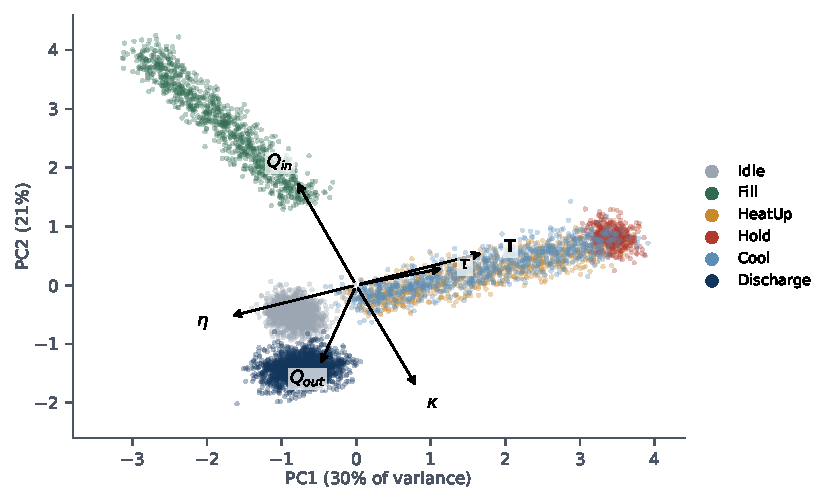
\includegraphics[width=\textwidth,height=0.68\textheight,keepaspectratio]{images/class14_pasteurization_pca_biplot.pdf}

\vspace{0.2em}
\begingroup\scriptsize\raggedright
PCA of 6{,}362 sensor samples (20 batches simulated with \texttt{synth\_sensors.py}, nine standardized variables); points are coloured by process phase and arrows show the loading of each sensor on PC1 and PC2. The phases form distinct regions even though the phase label was not used by PCA.
\par\endgroup
\coursefooter
\end{frame}

\begin{frame}{Embedding with PCA: a worked example (1/3)}
\begingroup\small
\textbf{Goal:} a $k = 2$ embedding of the $K = 6$ process phases, learned from sensor data (100 batches simulated with \texttt{synth\_sensors.py}).
\par\endgroup
\vspace{0.3em}
\centering
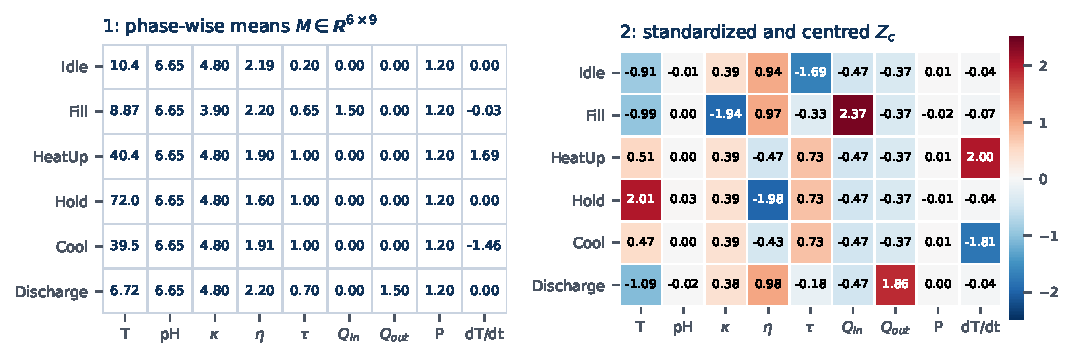
\includegraphics[width=\textwidth,height=0.47\textheight,keepaspectratio]{images/class14_pca_embedding_step12.pdf}

\vspace{0.2em}
\begin{itemize}\footnotesize
\item \textbf{Step 1:} each phase $v$ is described by the mean of nine sensor variables over its samples (row $\mathbf{m}_v$ of $M$).
\item \textbf{Step 2:} each sensor $j$ is standardized, $(m_{vj} - \mu_j)/\sigma_j$, so that variables in different units (°C, mS/cm, cP) become comparable; each column is then centred on the mean of the six phases, so that $0$ represents the average phase.
\end{itemize}
\coursefooter
\end{frame}

\begin{frame}{Embedding with PCA: a worked example (2/3)}
\begingroup\small
\textbf{Step 3:} PCA searches for new axes, each a weighted sum of the nine columns of $Z_c$, along which the phases differ as much as possible.
\par\endgroup
\vspace{0.3em}
\centering
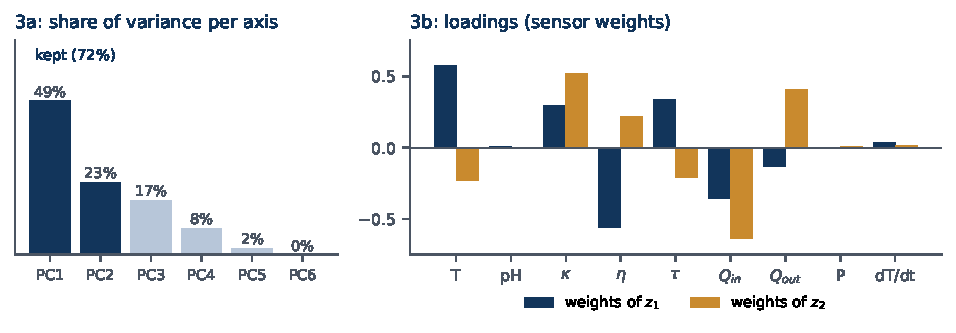
\includegraphics[width=0.92\textwidth,height=0.4\textheight,keepaspectratio]{images/class14_pca_embedding_step3.pdf}

\vspace{0.2em}
\begin{itemize}\footnotesize
\item \textbf{3a:} each bar is the share of the total variation between phases explained by one axis. The first two axes explain $49\% + 23\% = 72\%$, so we keep $k = 2$.
\item \textbf{3b:} the bars are the weights (loadings) of each sensor in the new axes.
$z_1$ weights temperature positively ($+0.58$) and viscosity $\eta$ negatively ($-0.56$): it is high for hot, thin milk, i.e.\ a \emph{temperature axis}.
$z_2$ weights inflow negatively and outflow and conductivity positively: it separates filling from discharge, i.e.\ a \emph{flow axis}.
pH and P receive weight $\approx 0$: they do not change between phases.
\end{itemize}
\coursefooter
\end{frame}

\begin{frame}{Embedding with PCA: a worked example (3/3)}
\begin{columns}[T]
\column{0.47\textwidth}
\centering
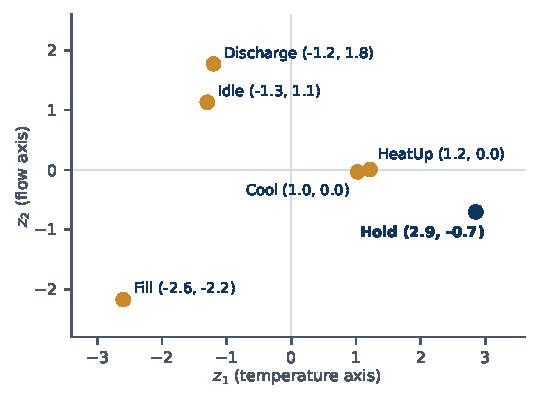
\includegraphics[width=\linewidth]{images/class14_pca_embedding_step4.pdf}
\column{0.51\textwidth}
\begingroup\small
\textbf{Step 4:} the coordinates of a phase are the weighted sums of its values in $Z_c$ (step 2, heatmap) with the weights of step 3b. For Hold:
\par\endgroup
\vspace{-0.2em}
\begingroup\footnotesize
\[
\begin{aligned}
z_1 &= \underbrace{0.58 \cdot 2.01}_{T} + \underbrace{(-0.56)(-1.98)}_{\eta} + \underbrace{0.34 \cdot 0.73}_{\tau} + \dots \\
&= 1.16 + 1.11 + 0.25 + \dots = 2.85
\end{aligned}
\]
\par\endgroup
\begingroup\footnotesize
Repeating this for every phase and for $z_2$ gives $E = Z_c W_2$: one point per phase.
\begin{itemize}\setlength{\itemsep}{1pt}
\item Close points mean similar sensor profiles.
\item Hold lies far right: the hottest phase.
\item Fill is isolated: the only phase with inflow.
\item HeatUp and Cool coincide: they differ only in dT/dt, which lies on PC3 (17\%) and is discarded with $k = 2$. This is the cost of compression.
\end{itemize}
\par\endgroup
\end{columns}
\coursefooter
\end{frame}

\begin{frame}{Papers and materials}
\readinglist{
\fontsize{6.8}{8.2}\selectfont
\begin{columns}[T]
\column{0.5\textwidth}
\begin{itemize}\setlength{\itemsep}{1pt}
\item Abiteboul, S. (1997). Querying semi-structured data. In \emph{Proceedings of the International Conference on Database Theory (ICDT)}, LNCS 1186, 1--18. Springer.
\item Zheng, A., Casari, A. (2018). \emph{Feature Engineering for Machine Learning}. O'Reilly.
\item Micci-Barreca, D. (2001). A preprocessing scheme for high-cardinality categorical attributes in classification and prediction problems. \emph{ACM SIGKDD Explorations}, 3(1), 27--32.
\item Jolliffe, I.\,T. (2002). \emph{Principal Component Analysis}, 2nd ed. Springer.
\item scikit-learn User Guide: \href{https://scikit-learn.org/stable/modules/preprocessing.html\#encoding-categorical-features}{encoding categorical features}; \href{https://scikit-learn.org/stable/modules/decomposition.html\#pca}{principal component analysis}.
\end{itemize}
\column{0.5\textwidth}
\begin{itemize}\setlength{\itemsep}{1pt}
\item Mikolov, T., Chen, K., Corrado, G., Dean, J. (2013). Efficient estimation of word representations in vector space. \href{https://arxiv.org/abs/1301.3781}{arXiv:1301.3781}.
\item Mikolov, T., Sutskever, I., Chen, K., Corrado, G., Dean, J. (2013). Distributed representations of words and phrases and their compositionality. \emph{Advances in Neural Information Processing Systems}, 26, 3111--3119.
\item Guo, C., Berkhahn, F. (2016). Entity embeddings of categorical variables. \href{https://arxiv.org/abs/1604.06737}{arXiv:1604.06737}.
\item Huyen, C. (2022). \emph{Designing Machine Learning Systems}. O'Reilly.
\end{itemize}
\end{columns}
}
\coursefooter
\end{frame}

\begin{frame}{Take-away message}
\vfill
\centering
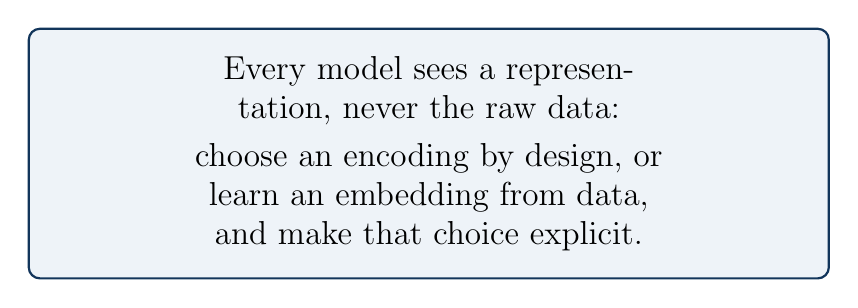
\begin{tikzpicture}
\node[fill=courseice, draw=courseblue, thick, rounded corners=4pt, inner sep=10pt, text width=0.78\textwidth, align=center, font=\large] {Every model sees a representation, never the raw data:\\[0.3em] choose an encoding by design, or learn an embedding from data,\\ and make that choice explicit.};
\end{tikzpicture}

\vfill
{\Large\bfseries\color{courseblue} Thank you for your attention.}

\vspace{0.4em}
{\small\color{coursegray} Next: Class 15 --- feature engineering: cleaning, curation, and selection.}
\vfill
\coursefooter
\end{frame}

\end{document}
